%Talk given at Monte Carlo Methods 2019
\documentclass[10pt,compress,xcolor={usenames,dvipsnames},aspectratio=169]{beamer}
%\documentclass[xcolor={usenames,dvipsnames},aspectratio=169]{beamer} %slides and 
%notes
\usepackage{amsmath,datetime,
	mathtools,
	bbm,
	%mathabx,
	array,
	booktabs,
	xspace,
	calc,
	colortbl,
 	graphicx}
\usepackage[usenames]{xcolor}
\usepackage[giveninits=false,backend=biber,style=nature, maxcitenames =10, mincitenames=9]{biblatex}
\addbibresource{FJHown23.bib}
\addbibresource{FJH23.bib}
\usepackage{newpxtext}
\usepackage[euler-digits,euler-hat-accent]{eulervm}
\usepackage{media9}
\usepackage[autolinebreaks]{mcode}
\usepackage[tikz]{mdframed}


\usetheme{FJHSlimNoFoot169}
\setlength{\parskip}{2ex}
\setlength{\arraycolsep}{0.5ex}

\DeclareMathOperator{\sol}{SOL}
\DeclareMathOperator{\app}{APP}
\DeclareMathOperator{\alg}{ALG}
\DeclareMathOperator{\ACQ}{ACQ}
\DeclareMathOperator{\ERR}{ERR}
\DeclareMathOperator{\COST}{COST}
\DeclareMathOperator{\COMP}{COMP}
\newcommand{\dataN}{\bigl(\hf(\vk_i)\bigr)_{i=1}^n}
\newcommand{\dataNj}{\bigl(\hf(\vk_i)\bigr)_{i=1}^{n_j}}
\newcommand{\dataNjd}{\bigl(\hf(\vk_i)\bigr)_{i=1}^{n_{j^\dagger}}}
\newcommand{\ERRN}{\ERR\bigl(\dataN,n\bigr)}

\newcommand{\Sapp}{S_{\textup{app}}}
\newcommand{\LambdaStd}{\Lambda^{\textup{std}}}
\newcommand{\LambdaSer}{\Lambda^{\textup{ser}}}
\newcommand{\LambdaAll}{\Lambda^{\textup{all}}}
%\DeclareMathOperator{\spann}{span}
%\DeclareMathOperator{\app}{app}

\providecommand{\HickernellFJ}{H.}


\iffalse
Adaptive Approximation to Multivariate Linear Problems with Inputs Lying in a Cone

Adaptive algorithms are convenient for the practitioner because they automatically determine the computational effort required to satisfy the error criterion.  The function data acquired for constructing the approximate solution are also used to compute a data-based error bound for the approximate solution.  Computation proceeds until this error bound becomes small enough.  If the set of allowed input functions is convex, adaptive algorithms may offer no advantage to non-adaptive algorithms.  We construct an adaptive algorithm for solving a general, linear problem where the input functions lie in a  \emph{non-convex cone}. The stopping criterion is based on theory, not heuristics.  The cone of input functions is defined so that sampling the most important Fourier series coefficients is sufficient to bound the magnitude of the unsampled Fourier coefficients.  We show that our adaptive algorithm is optimal.  We also determine conditions under which the problem is tractable.  This work is related to  the adaptive algorithms developed in \cite{HicEtal14a,HicEtal17a,KunEtal19a}.

\fi

\renewcommand{\OffTitleLength}{-10ex}
\setlength{\FJHThankYouMessageOffset}{-8ex}
\title{The Right Ingredients for \\ Adaptive Function Approximation Algorithms}
\author[]{Fred J. Hickernell}
\institute{Department of Applied Mathematics \\
	Center for Interdisciplinary Scientific Computation \\  Illinois Institute of Technology \\
	\href{mailto:hickernell@iit.edu}{\url{hickernell@iit.edu}} \quad
	\href{http://mypages.iit.edu/~hickernell}{\url{mypages.iit.edu/~hickernell}}}

\thanksnote{with Yuhan Ding, Mac Hyman, Peter Kritzer, and Simon Mak \\
	partially supported by  NSF-DMS-1522687 and NSF-DMS-1638521 (SAMSI)
}
\event{Old Dominion University}
\date[]{March 6, 2020}

\input FJHDef.tex


%Abstract:  When

\newlength{\figwidth}
\setlength{\figwidth}{0.25\textwidth}

\newlength{\figwidthSmall}
\setlength{\figwidthSmall}{0.2\textwidth}

\newcommand{\financePict}{\href{http://i2.cdn.turner.com/money/dam/assets/130611131918-chicago-board-options-exchange-1024x576.jpg}{\includegraphics[width
		= 3cm]{ProgramsImages/130611131918-chicago-board-options-exchange-1024x576.jpg}}}
	
	\newcommand{\scoop}[1]{\parbox{#1}{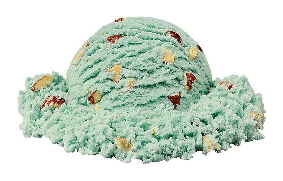
\includegraphics[width=#1]{IceCreamScoop.eps}}\xspace}
	\newcommand{\smallscoop}{\scoop{1cm}}
	\newcommand{\medscoop}{\scoop{1.8cm}}
	\newcommand{\largescoop}{\scoop{3cm}}
	\newcommand{\ICcone}[1]{\parbox{#1}{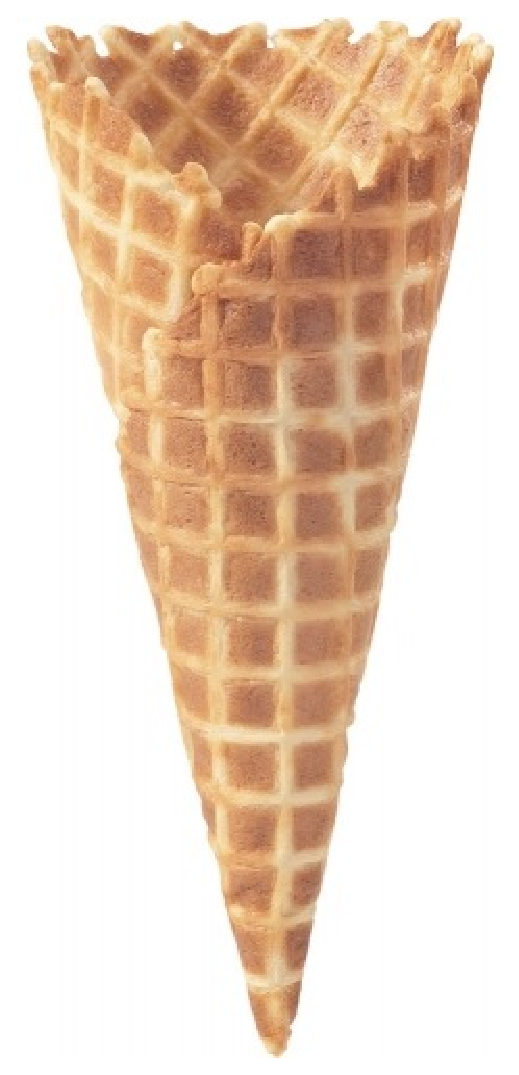
\includegraphics[width=#1,angle=270]{MediumWaffleCone.eps}}\xspace}
	\newcommand{\medcone}{\ICcone{1.2cm}}
	\newcommand{\largercone}{\parbox{2.2cm}{\vspace*{-0.2cm}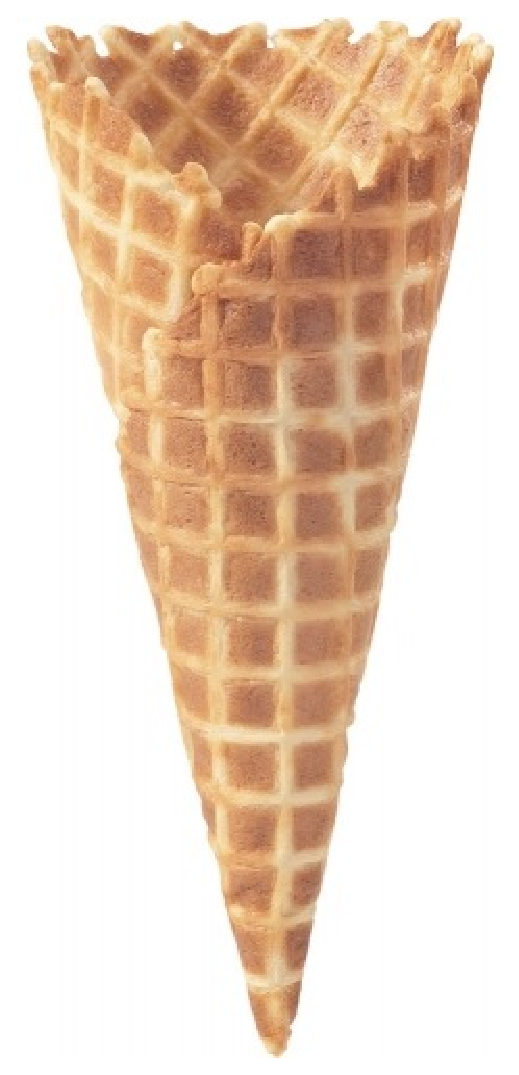
\includegraphics[width=1cm,angle=270]{MediumWaffleCone.eps}}\xspace}
	\newcommand{\largecone}{\ICcone{1.8cm}}
	\newcommand{\smallcone}{\parbox{1.1cm}{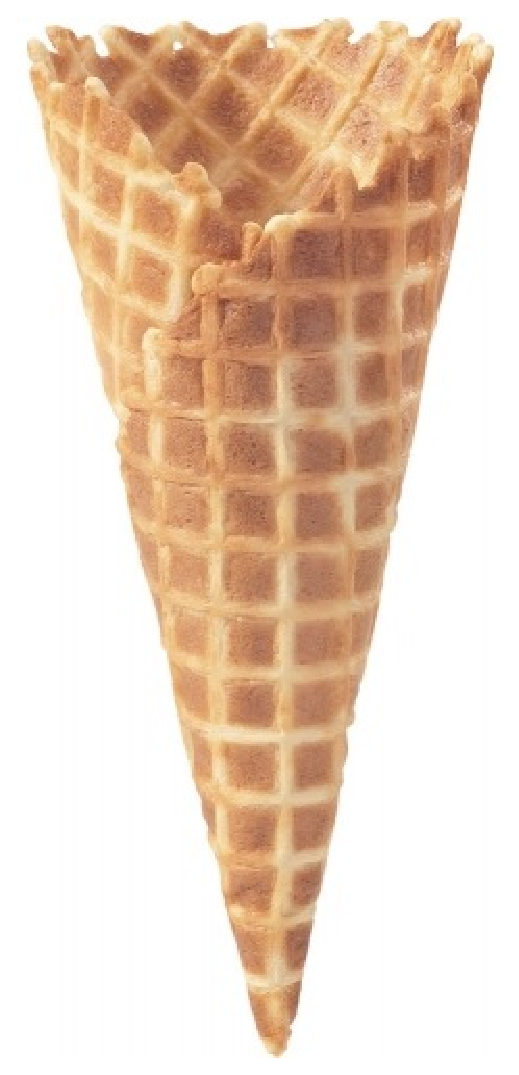
\includegraphics[width=0.5cm,angle=270]{MediumWaffleCone.eps}}\xspace}

	

\newcommand{\northeaststuff}[3]{
	\begin{tikzpicture}[remember picture, overlay]
	\node [shift={(-#1 cm,-#2 cm)}]  at (current page.north east){#3};
	\end{tikzpicture}}


\begin{document}
	\tikzstyle{every picture}+=[remember picture]
	\everymath{\displaystyle}

\frame{\titlepage}


\section{Introduction}

\begin{frame}{Problem}

\vspace{-5ex}
\begin{itemize}
    \item Have a \alert{black-box} function routine $f \colon \Omega \subseteq \reals^d \to \reals$, e.g., output of a computer simulation
    
    \item Cost of a function value, $\$(f)$, is \alert{expensive}
    
    \item Want \alert{fixed tolerance algorithm} $\alg: \cc \times (0,\infty) \to \cg$ such that 
    \[
    \norm[\cg]{f - \alg(f,\varepsilon)} \le \varepsilon \qquad \forall f \in \cc \text{ \alert{candidate set}}, \quad \cc \subset \cg \alert{\text{ Banach space}}
    \]
    cost of an $\alg(f,\varepsilon)$ value is \alert{cheap}\uncover<2->{
    \begin{gather*}
        \text{\alert{design or node array} }\mX \in \Omega^n \subseteq \reals^{n \times d}, \qquad \text{\alert{function data} }  \vy = f(\mX)\in \reals^n \\
        \vx_{n+1} = \argmax_{\vx \in \Omega} \ACQ(\vx,n,\mX,\vy) \text{ \alert{acquisition function}} \\
        \norm[\cg]{f - \app(n,\mX,\vy)} \le \ERR(n,\mX,\vy) \text{ \alert{data-driven error bound}} \qquad \forall n \in \naturals, \ f \in \cc \\
        n^* = \min \, \{ n \in \naturals \colon \ERR(n,\mX,\vy) \le \varepsilon \} \text{ \alert{stopping criterion}} \\
        \alg(f,\varepsilon) = \app(n^*,\mX,\vy) \text{ \alert{fixed budget approximation}}
    \end{gather*}}
 \end{itemize}
 
 \vspace{-4ex}
 \uncover<2->{\alert{Adaptive} sample size, design, and fixed budget approximation}
    
\end{frame}


\section{Univariate, Low Accuracy}

\begin{frame}{Linear Splines}
\begin{align*}
    f & :[a,b] \to \reals, \qquad a =: x_0 < x_1 < \cdots < x_n :=b, \qquad \vy = f(\vx) \\
    \app(n,\vx,\vy) & := \frac{x -x_i}{x_{i-1} - x_i} y_{i-1} +  \frac{x -x_{i-1}}{x_i - x_{i-1}} y_{i}, \quad x_{i-1} \le x \le x_i, \qquad \alert{\text{linear spline}} \\
    \norm[{\infty,[x_{i-1}, x_i]}]{f - \app(n,\vx,\vy)} & \le 
\end{align*}
    
\end{frame}





\begin{frame}{Context}

\vspace{-5ex}

\begin{itemize}
	\item Linear \alert{solution} operator $\sol : \cf \to \cg$, input space $\cf$ contains functions defined on $\Omega \subseteq \reals^d$ \\
	\qquad e.g., $\sol(f) = f$, \quad $- \nabla^2 \sol(f) = f, \  \sol(f) = 0$  on boundary
	\item \alert{Approximation} $\app(f,n) = \sum_{i=1}^n L_i(f) g_i$, can sample linear functionals \\
	\qquad $\norm[\cg]{\sol(f) - \app(f,n)} \le \norm[\cf \to \cg]{\sol - \app(\cdot,n)} \norm[\cf]{f}$
	\item \alert{Algorithm} $\alg(f,\varepsilon) = \app\bigl(f,n^*(f,\varepsilon)\bigr)$ satisfying  
	$\norm[\cg]{\sol(f) - \alg(f,\varepsilon)} \le \varepsilon$ for all $f \in \alert{\cc} \subset \cf$

\uncover<2->{\item \alert{Solvability:} what $\cc$?  how  to determine $n^*(f,\varepsilon) \in \naturals$?  
	\only<3->{\smallscoop\only<3->{\hspace{-6.5ex}\raisebox{-1.5ex}{\color{red}\fontsize{40}{48}\selectfont $\times$}} or \smallcone}
\only<2>{
	
	\begin{itemize}
	\item $n^*(f,\varepsilon) = \min\{n : \norm[\cf \to \cg]{\sol - \app(\cdot,n)} \le \varepsilon / R\}$  if $f \in \smallscoop$ of radius $R$
	
	\item Alternatively, assume $f \in \smallcone$ and bound $ \norm[\cf]{f}$ or equivalent\footfullcite{HicEtal17a,KunEtal19a,DinHic20a} \\
	\emph{What you do not see is not much worse than what you see?}
\end{itemize}}

\only<3->{\item \alert{Optimality:} is $n^*(f,\varepsilon)$ essentially as small as possible?
	
	\item \alert{Tractability:} does $n^*(f,\varepsilon)$ depend nicely on $d$?
}
}

\end{itemize}

\end{frame}

\end{document}


\section{Algorithm}

\begin{frame}<1>[label = Setup]{
		\only<1>{General Linear Problems Defined on Series Spaces}%
		\only<2-4>{Adaptive Algorithm for General Linear Problems on Cone of Inputs}%
		\only<5>{Optimality of Algorithm}%
		\only<6>{Tractability  of Solving General Linear Problems on Cone of Inputs}%
		\footfullcite{DinEtal20a}}
	
	\vspace{-7ex}
	
	\begin{align*}
	\only<1-2>{
        \cf &:= \left \{ f = \sum_{i=1}^\infty \hf(\vk_i) u_{\vk_i} : \norm[\cf]{f} := \norm[\rho]{\left(\frac{\bigabs{\hf(\vk_i)}}{\lambda_{\vk_i}} \right)_{i =1}^\infty} \right \} \qquad 
		\begin{minipage}{4.2cm}\raggedright  
		    $\lambda_{\vk_1} \ge \lambda_{\vk_2} \ge \cdots > 0$ \\
		    \alert{$\vlambda$ affects convergence rate \&  \\ tractability}
		\end{minipage}\\
		\cg &: = \biggl \{ g = \sum_{i=1}^\infty \hg(\vk_i) v_{\vk_i} : \norm[\cg]{g} := \bignorm[\tau]{\hg}\biggr \}, \qquad
		\sol(f) = \sum_{i=1}^\infty \hf(\vk_i) v_{\vk_i}, \quad \tau \le \rho \\
		}
	    \uncover<2->{\cc_{\only<6>{\alert{d},}\only<1-5>{\vlambda}\only<6>{\alert{\vlambda_d}}, n_1, A} &: = \Biggl\{ f \in \cf : \norm[\cf]{f} \le A\norm[\rho]{\biggl ( \frac{\hf(\vk_i) }{\lambda_{\vk_i}} \biggr) _{i=1}^{n_1}} \Biggr\} \qquad 
		\begin{minipage}{5.5cm}\raggedright 
		    \alert{pilot sample \\ bounds the norm of the input}
		\end{minipage} }
        \only<2-4>{\uncover<2-4>{\\
	        \app(f,n) &= \sum_{i=1}^{n} \hf(\vk_i) v_{\vk_i}\quad  \alert{\text{optimal for fixed }n}
	        \qquad \norm[\cg]{\sol(f) - \app(f,n)} \le  \ERRN 
	        }}
		\end{align*}
		\vspace{-2ex}
\only<2-4>{\uncover<2-4>{\begin{equation*}
    \ERRN := \underbrace{\left[ A^\rho \norm[\rho]{\left( \frac{\hf(\vk_i)}{\lambda_{\vk_i}} \right)_{i=1}^{n_1}}^\rho -  \norm[\rho]{\left(\frac{\hf(\vk_i)}{\lambda_{\vk_i}}\right)_{i=1}^n}^\rho \right]^{1/\rho}}_{\text{upper bound on } \norm[\cf]{f - \sum_{i=1}^{n} \hf(\vk_i) u_{\vk_i}}}
    \, 
    \underbrace{\bignorm[\rho']{\bigl( \lambda_{\vk_i}  \bigr)_{i = n+1}^{\infty}}}_{\norm[\cf \to \cg]{\sol - \app(\cdot,n)}}  
    \quad 
\begin{minipage}{2cm}
    $\displaystyle \frac 1\rho + \frac 1 {\rho'} = \frac 1 \tau $\\[1ex]
    \alert{\text{data-driven}}
\end{minipage}
\end{equation*}
}}
    \only<3-5>{\vspace{-2ex}
    \begin{align*}
	\alert<3>{\alg(f,\varepsilon)} & 
	\alert<3>{= \app(f,n^*(f,\varepsilon))} 
	\text{ for } \alert<3>{n^*(f,\varepsilon) = \min \{ n \in \naturals : \ERRN \le \varepsilon\} }
	\\ 
    \uncover<4->{
    \alert<4>{\COST(\alg,\cc_{\vlambda, n_1,A},\varepsilon,R)} 
    & \alert<4>{= \max \bigl \{ n^*(f,\varepsilon) : f \in \cc_{\vlambda, n_1, A} \cap \cb_R = \smallcone \cap \smallscoop \bigr\}} \\
    & \alert<4>{= \min \left \{n \ge n_1 : \bignorm[\rho']{\bigl(  \lambda_{\vk_i}  \bigr)_{i = n+1}^{\infty}} \,
    \le \varepsilon/[(A^\rho -1)^{1/\rho}R] \right \}}
		}
	\only<5->{ \\
	\alert{\COMP(\ca(\cc_{\vlambda, n_1,A},\varepsilon,R))} & = \min \{\COST(\alg',\cc_{\vlambda, n_1,A},\varepsilon,R)  : \alg' \in   \ca(\cc_{\vlambda, n_1,A})    \} \\
	& \ge \alert{\COST(\alg,\cc_{\vlambda, n_1,A},\omega \varepsilon,R)}, \qquad 
	\omega = \frac{2A(A^\rho -1)^{1/\rho}}{A - 1} > 1\\
	& \qquad \qquad \text{\alert{via fooling functions}}
	}
    \end{align*}
    \only<5>{$\alg$ is \alert{essentially optimal}}
    }
    \only<6>{For $\tau = \rho$ ($\rho'=\infty$), the problem $\sol_d :\cc_{\alert{d},\alert{\vlambda_d}, n_1, A} \to \cg_d$ is 
    \begin{description}
    \item[Strongly polynomial tractable] iff there exist $i_0 \in \naturals$ and $\eta > 0$ such that \quad
    $\displaystyle  \sup_{d\in\naturals} \sum_{i=i_0}^\infty \lambda_{d,\vk_i}^\eta < \infty$
    
    \item[Polynomial tractable] iff there exist $\eta_1, \eta_2 \ge 0$ and $\eta_3, K>0$ such that \qquad
 $
    \sup_{d\in\naturals} d^{-\eta_1}\, \sum_{i=\lceil K d^{\eta_2} \rceil}^\infty \lambda_{d,\vk_i}^{\eta_3} < \infty
 $
 \item[Weakly tractable] iff \quad
 $
  \sup_{d\in\naturals} \, \exp(-cd) \sum_{i=1}^\infty \exp\left(-c\left(\frac{1}{\lambda_{d,\vk_i}}\right)\right) <\infty$ \; for all $c>0$
 
    \end{description}
    Analogous results exist for $ \tau < \rho$ ($\rho' < \infty$)
    }

	
\end{frame}


\begin{frame}{Legendre and Chebyshev Bases for Function Approximation}
\vspace{-3ex}
	\begin{tabular}{>{\centering}m{0.18\textwidth}>{\centering}m{0.18\textwidth}>{\centering}m{0.18\textwidth}>{\centering}m{0.18\textwidth}>{\centering}m{0.18\textwidth}}
		\includegraphics[width =0.18\textwidth]{ProgramsImages/Legendre_Degree_0.png}  &
		\includegraphics[width =0.18\textwidth]{ProgramsImages/Legendre_Degree_1.png}  &
		\includegraphics[width =0.18\textwidth]{ProgramsImages/Legendre_Degree_2.png}  &
		\includegraphics[width =0.18\textwidth]{ProgramsImages/Legendre_Degree_3.png}  &
		\includegraphics[width =0.18\textwidth]{ProgramsImages/Legendre_Degree_4.png} 
	\tabularnewline[-7ex]
	Legendre
	\tabularnewline
	\tabularnewline
		\includegraphics[width =0.18\textwidth]{ProgramsImages/Legendre_Degree_1_1.png}  &
\includegraphics[width =0.18\textwidth]{ProgramsImages/Legendre_Degree_1_2.png}  &
\includegraphics[width =0.18\textwidth]{ProgramsImages/Legendre_Degree_1_3.png}  &
\includegraphics[width =0.18\textwidth]{ProgramsImages/Legendre_Degree_2_2.png}  &
\includegraphics[width =0.18\textwidth]{ProgramsImages/Legendre_Degree_2_3.png} 
\tabularnewline[0ex]
		\includegraphics[width =0.18\textwidth]{ProgramsImages/Chebyshev_Degree_0.png}  &
\includegraphics[width =0.18\textwidth]{ProgramsImages/Chebyshev_Degree_1.png}  &
\includegraphics[width =0.18\textwidth]{ProgramsImages/Chebyshev_Degree_2.png}  &
\includegraphics[width =0.18\textwidth]{ProgramsImages/Chebyshev_Degree_3.png}  &
\includegraphics[width =0.18\textwidth]{ProgramsImages/Chebyshev_Degree_4.png} 
\tabularnewline[-7ex]
Chebyshev \tabularnewline
\tabularnewline
\includegraphics[width =0.18\textwidth]{ProgramsImages/Chebyshev_Degree_1_1.png}  &
\includegraphics[width =0.18\textwidth]{ProgramsImages/Chebyshev_Degree_1_2.png}  &
\includegraphics[width =0.18\textwidth]{ProgramsImages/Chebyshev_Degree_1_3.png}  &
\includegraphics[width =0.18\textwidth]{ProgramsImages/Chebyshev_Degree_2_2.png}  &
\includegraphics[width =0.18\textwidth]{ProgramsImages/Chebyshev_Degree_2_3.png} 
	\end{tabular}
\end{frame}

\againframe<2-4>{Setup}

\section{Optimality}

\againframe<5>{Setup}

\section{Tractability}

\againframe<6->{Setup}

\section{Alternate Cone}

\begin{frame}
	\frametitle{An Alternate Cone, Similar to Our Cone}
	\vspace{-5.5ex}
	\begin{gather*}
	\norm[\cf]{f} : = \norm[\rho]{\biggl ( \frac{\hf(\vk_i) }{\lambda_{\vk_i}} \biggr) _{i=1}^\infty}, \quad \lambda_{\vk_i} \downarrow 0, \qquad
	\norm[\cf']{f} : = \norm[\rho]{\biggl ( \frac{\hf(\vk_i) \zeta_{\vk_i}}{\lambda_{\vk_i}} \biggr) _{i=1}^\infty},  
	\quad \zeta_{\vk_1} = 1, \; \zeta_{\vk_i} \downarrow
\\
	\underbrace{\cc_{\vlambda, n_1, A} : = \Biggl\{ f \in \cf : \norm[\cf]{f} \le A\norm[\rho]{\biggl ( \frac{\hf(\vk_i) }{\lambda_{\vk_i}} \biggr) _{i=1}^{n_1}} \Biggr\} }_{\text{pilot sample bounds the norm of the input}}
	\qquad 
	\alert{\underbrace{\cc'_{\vlambda, \vzeta, A'} : = \bigl \{ f \in \cf : \norm[\cf]{f} \le A'\norm[\cf']{f} \bigr \} }_{\text{stronger norm is bounded above by weaker norm}}}
	\end{gather*}

		\begin{gather*}
\alert{\cc'_{\vlambda, \vzeta, A'} \subseteq \cc_{\vlambda, n_1, A}}  \qquad 
\text{for } A \ge A'\left[\frac{1 + \zeta_{\vk_{n_1+1}}^\rho}{1 - (\zeta_{\vk_{n_1+1}}A')^\rho}\right]^{1/\rho},  \quad \zeta_{\vk_{n_1+1}}A' < 1  \\
\alert{\cc_{\vlambda, n_1, A} \subseteq \cc'_{\vlambda, \vzeta, A''} }  \qquad 
\text{for } A \le A'' \zeta_{\vk_{n_1}}
		\end{gather*}

\end{frame}



\begin{frame}
	\frametitle{An Alternative Cone, Similar to Our Cone}
	\vspace{-2ex}
	For any $f \in 	\cc'_{\vlambda, \vzeta, A'} $ it follows that 
	\begin{align*}
	\norm[\cf']{f}^\rho- \norm[\rho]{\biggl ( \frac{\hf(\vk_i) \zeta_{\vk_i} }{\lambda_{\vk_i}} \biggr) _{i=1}^{n_1}}^\rho 
	& = \norm[\rho]{\biggl ( \frac{\hf(\vk_i) \zeta_{\vk_i} }{\lambda_{\vk_i}} \biggr) _{i=n_1 + 1}^{\infty}}^\rho \\
	& \le \zeta_{\vk_{n_1 +1}}^\rho \norm[\rho]{\biggl ( \frac{\hf(\vk_i) }{\lambda_{\vk_i}} \biggr) _{i=n_1 + 1}^{\infty}}^\rho 
	= \zeta_{\vk_{n_1 +1}}^\rho \left[ \norm[\cf]{f}^\rho - \norm[\rho]{\biggl ( \frac{\hf(\vk_i) }{\lambda_{\vk_i}} \biggr) _{i=1}^{n_1}}^\rho \right ]\\	
	& \le \zeta_{\vk_{n_1 +1}}^\rho \left[ A'{}^\rho \norm[\cf']{f}^\rho -  \norm[\rho]{\biggl ( \frac{\hf(\vk_i) \zeta_{\vk_i}}{\lambda_{\vk_i}} \biggr) _{i=1}^{n_1}}^\rho \right ]
	\uncover<2>{\\
		\norm[\cf']{f}^\rho & \le \frac{1 + \zeta_{\vk_{n_1 +1}}^\rho}{1 - (\zeta_{\vk_{n_1 +1}}A')^\rho} \norm[\rho]{\biggl ( \frac{\hf(\vk_i) \zeta_{\vk_i} }{\lambda_{\vk_i}} \biggr) _{i=1}^{n_1}}^\rho \\
		\norm[\cf]{f} & \le A' \norm[\cf']{f} 
		\le A'\left[\frac{1 + \zeta_{\vk_{n_1 +1}}^\rho}{1 - (\zeta_{\vk_{n_1 +1}}A')^\rho}\right]^{1/\rho} \norm[\rho]{\biggl ( \frac{\hf(\vk_i)}{\lambda_{\vk_i}} \biggr) _{i=1}^{n_1}}
	}
	\end{align*}
\end{frame}


\begin{frame}
	\frametitle{An Alternate Cone, Similar to Our Cone}
	\vspace{-2ex}
	For any $f \in \cc_{\vlambda, n_1, A} $ it follows that 
	\begin{equation*}
\norm[\cf]{f} \le A \norm[\rho]{\biggl ( \frac{\hf(\vk_i)}{\lambda_{\vk_i}} \biggr) _{i=1}^{n_1}} 
    \le  \frac{A}{\zeta_{\vk_{n_1}}} \norm[\rho]{\biggl ( \frac{\hf(\vk_i) \zeta_{\vk_i} }{\lambda_{\vk_i}} \biggr) _{i=1}^{n_1}}
    \le \frac{A}{\zeta_{\vk_{n_1}}} \norm[\cf']{f}
	\end{equation*}
\end{frame}

\section{Summary}

\begin{frame}
	\frametitle{Conclusion}
	
	\vspace{-4ex}
	
	\alert{Summary}
	
	\vspace{-3ex}
	\begin{itemize}
		\item Adaptive algorithms can be constructed for non-convex, symmetric cones of inputs
		
		\item One possible cone assumes that a pilot sample tells you enough about the norm of the input
		
		\item Information cost and complexity depend on the norm of the input, but the adaptive algorithm does not  know this norm
		
		\item There are tractability results for problems defined on cones
		
		\item Our algorithm can be extended to infer the $\lambda_{\vk}$ in terms of coordinate weights\footfullcite{DinEtal20a}
	\end{itemize}

\alert{Further Work}

	\vspace{-3ex}
	\begin{itemize}
	\item Need to develop and analyze algorithms based on function values, not series coefficients
	
\end{itemize}


\end{frame}

\begin{frame}{Cheng and Sandu Function\footfullcite{VirLib17a}}
	\vspace{-9ex}
	\begin{gather*}
	\text{Function values for data \qquad Chebyshev polynomial basis}, \qquad \lambda_{\vk} \text{ \alert{inferred} }, 
	\end{gather*}
	
	
	\centerline{\includegraphics[height = 5cm]{ProgramsImages/sim_eval_results_chsan10_d6_sflg0ErrN.eps}}
	
\end{frame}



\finalthanksnote{These slides are  available at \\  \href{https://speakerdeck.com/fjhickernell/mcm-2019-pilot-sample}{\nolinkurl{speakerdeck.com/fjhickernell/mcm-2019-pilot-sample}}}


\thankyouframe

\begin{frame}[allowframebreaks]
	\frametitle{References}
\printbibliography
\end{frame}




\end{document}



